Classic GHZ question.
\begin{parts}
	\part Want eigenstates of $\mathrm{X}$ and $\mathrm{Y}$:
	\begin{equation*}
		\sigma_x = \begin{pmatrix}
			0 & 1 \\
			1 & 0
		\end{pmatrix}
		\Rightarrow \textnormal{\hspace{1em}Seek\hspace{1em}} \begin{vmatrix}
			-\lambda & 1 \\
			1 & -\lambda
		\end{vmatrix} = 0
		\Rightarrow \lambda = \pm 1
	\end{equation*}
	\begin{align*}
		\Rightarrow \textnormal{\hspace{1em}Eigenstates\hspace{1em}} \ket{\mathrm{H}^\prime} &= \frac{\ket{\mathrm{H}}+\ket{\mathrm{V}}}{\sqrt{2}} \\
		\ket{\mathrm{V}^\prime} &= \frac{\ket{\mathrm{H}}-\ket{\mathrm{V}}}{\sqrt{2}}
	\end{align*}
	
	Similarly,
	\begin{equation*}
		\sigma_y = \begin{pmatrix}
			0 & i \\
			-i & 0
		\end{pmatrix}
		\Rightarrow \textnormal{\hspace{1em}Seek\hspace{1em}} \begin{vmatrix}
			-\lambda & i \\
			-i & -\lambda
		\end{vmatrix} = 0
		\Rightarrow \lambda = \pm i
	\end{equation*}
	\begin{align*}
		\Rightarrow \textnormal{\hspace{1em}Eigenstates\hspace{1em}} \ket{\mathrm{R}} &= \frac{\ket{\mathrm{H}}+i\ket{\mathrm{V}}}{\sqrt{2}} \\
		\ket{\mathrm{L}} &= \frac{\ket{\mathrm{H}}-i\ket{\mathrm{V}}}{\sqrt{2}}
	\end{align*}
	
	Note that in optics the correspondence are $\{\ket{\mathrm{H}^\prime},\,\ket{\mathrm{V}^\prime}\}\equiv$ linear polarisation \SI{45}{\degree} to the $\{\ket{\mathrm{H}},\,\ket{\mathrm{V}}\}$ axes, and $\{\ket{\mathrm{R}},\,\ket{\mathrm{L}}\}\equiv$ right/left-handed polarisation.
	
	To measure these polarisation, consider the following setup:
	\begin{figure}[H]
		\centering
		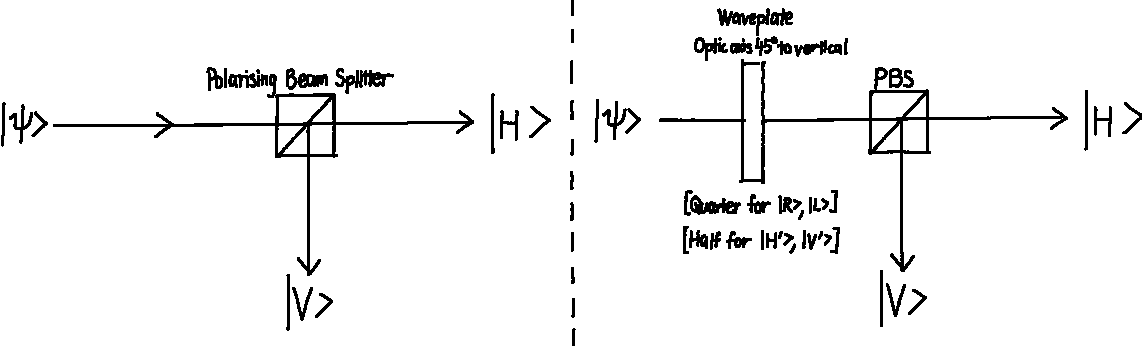
\includegraphics[width=.85\linewidth]{q6-polarisation}
	\end{figure}
	
	\part $\ket{\textnormal{GHZ}} = \diagfrac{1}{\sqrt{2}}\left[\ket{\textnormal{HHH}}-i\ket{\textnormal{VVV}}\right]$
	
	Noting orthogonality between the basis, we have:
	\begin{gather*}
		P(\textnormal{HHH}) = P(\textnormal{VVV}) = \left|\frac{1}{\sqrt{2}}\right|^2 = \left|-\frac{i}{\sqrt{2}}\right|^2 = \frac{1}{2} \\
		P(\textnormal{HHV}) = P(\textnormal{HVH}) = \ldots = 0
	\end{gather*}
	
	From above, we have for X basis:
	\begin{gather*}
		\ket{\mathrm{H}} = \frac{\ket{\mathrm{H}^\prime} + \ket{\mathrm{V}^\prime}}{\sqrt{2}} \\
		\ket{\mathrm{V}} = \frac{\ket{\mathrm{H}^\prime} - \ket{\mathrm{V}^\prime}}{\sqrt{2}}
	\end{gather*}
	
	For Y basis:
	\begin{gather*}
		\ket{\mathrm{H}} = \frac{\ket{\mathrm{R}} + \ket{\mathrm{L}}}{\sqrt{2}} \\
		\ket{\mathrm{V}} = -i\frac{\ket{\mathrm{R}} - \ket{\mathrm{L}}}{\sqrt{2}}
	\end{gather*}
	
	\begin{align*}
		\textnormal{So } \ket{\textnormal{GHZ}} &= \frac{1}{\sqrt{2}} \left[\left(\frac{\ket{\mathrm{H}^\prime} + \ket{\mathrm{V}^\prime}}{\sqrt{2}}\right)^{\otimes 2} \left(\frac{\ket{\mathrm{R}} + \ket{\mathrm{L}}}{\sqrt{2}}\right)
		-i \left(\frac{\ket{\mathrm{H}^\prime} - \ket{\mathrm{V}^\prime}}{\sqrt{2}}\right)^{\otimes 2} \left(-i\frac{\ket{\mathrm{R}} - \ket{\mathrm{L}}}{\sqrt{2}}\right)\right] \\
		&= \frac{1}{4} \Bigl[\bigl(\ket{\mathrm{H}^\prime}+\ket{\mathrm{V}^\prime}\bigr) \bigl(\ket{\mathrm{H}^\prime}+\ket{\mathrm{V}^\prime}\bigr) \bigl(\ket{\mathrm{R}}+\ket{\mathrm{L}}\bigr) \\
		&\phantom{=\frac{1}{4}} - \bigl(\ket{\mathrm{H}^\prime}-\ket{\mathrm{V}^\prime}\bigr) \bigl(\ket{\mathrm{H}^\prime}-\ket{\mathrm{V}^\prime}\bigr) \bigl(\ket{\mathrm{R}}-\ket{\mathrm{L}}\bigr)\Bigr] \\
	\end{align*}
	
	Noting that most cross terms vanish but those with matching parity, we have:
	\begin{align*}
		\ket{\textnormal{GHZ}} &= \frac{1}{4} \Bigl[\ket{\mathrm{H}^\prime \mathrm{H}^\prime \mathrm{L}} + \ket{\mathrm{V}^\prime \mathrm{V}^\prime \mathrm{L}} + \ket{\mathrm{H}^\prime \mathrm{V}^\prime \mathrm{R}} + \ket{\mathrm{V}^\prime \mathrm{H}^\prime \mathrm{R}}\Bigr] \times 2 \\
		&= \frac{1}{2}\Bigl[\ldots\Bigr]
	\end{align*}
	
	Noting the similarity in parity matching, we simply swap label for XYX and YXX:
	\begin{equation*}
		\ket{\textnormal{GHZ}} = 
		\begin{cases}
			\diagfrac{1}{2} \bigl[\ket{\mathrm{H}^\prime \mathrm{L} \mathrm{H}^\prime} + \ket{\mathrm{V}^\prime \mathrm{L} \mathrm{V}^\prime} + \ket{\mathrm{H}^\prime \mathrm{R} \mathrm{V}^\prime} + \ket{\mathrm{V}^\prime \mathrm{R} \mathrm{H}^\prime}\bigr] &\textnormal{XYX} \\
			\diagfrac{1}{2} \bigl[\ket{\mathrm{L} \mathrm{H}^\prime \mathrm{H}^\prime} + \ket{\mathrm{L} \mathrm{V}^\prime \mathrm{V}^\prime} + \ket{\mathrm{R} \mathrm{H}^\prime \mathrm{V}^\prime} + \ket{\mathrm{R} \mathrm{V}^\prime \mathrm{H}^\prime}\bigr] &\textnormal{YXX}
		\end{cases}
	\end{equation*}
	
	The possible outcomes are then:
	
	XXY: $\ket{\mathrm{H}^\prime \mathrm{H}^\prime \mathrm{L}}$, $\ket{\mathrm{V}^\prime \mathrm{V}^\prime \mathrm{L}}$, $\ket{\mathrm{H}^\prime \mathrm{V}^\prime \mathrm{R}}$, $\ket{\mathrm{V}^\prime \mathrm{H}^\prime \mathrm{R}}$ each with probability of $|\diagfrac{1}{2}|^2 = \diagfrac{1}{4}$.
	
	Similar results follow for XYX and YXX.
	
	\part Following local realism, we observe that there is an element of anti-correlation between the first and second qubit when the third qubit is $\ket{\mathrm{R}}$, correlation when the third qubit is $\ket{\mathrm{L}}$.
	Hence in YYY basis we expect to have results $\ket{\textnormal{LRR}}$, $\ket{\textnormal{RLR}}$, $\ket{\textnormal{RRL}}$, $\ket{\textnormal{LLL}}$ each with probability $\diagfrac{1}{4}$.
	
	Now let's rewrite the state in YYY basis:
	\begin{equation*}
		\ket{\textnormal{GHZ}} = \frac{1}{4} \Bigl[\left(\ket{\mathrm{R}}+\ket{\mathrm{L}}\right)\left(\ket{\mathrm{R}}+\ket{\mathrm{L}}\right)\left(\ket{\mathrm{R}}+\ket{\mathrm{L}}\right)
		-i\left(\ket{\mathrm{R}}-\ket{\mathrm{L}}\right)\left(\ket{\mathrm{R}}-\ket{\mathrm{L}}\right)\left(\ket{\mathrm{R}}-\ket{\mathrm{L}}\right)\left(-i\right)^3\Bigr]
	\end{equation*}
	
	Noting the opposite parity requirement, we have:
	\begin{equation*}
		\ket{\textnormal{GHZ}} = \frac{1}{4} \bigl[\ket{\textnormal{RRR}} + \ket{\textnormal{LLR}} + \ket{\textnormal{LRL}} + \ket{\textnormal{RLL}}\bigr] \times 2
	\end{equation*}
	
	But here we yield a different set of outcomes: $\ket{\textnormal{RRR}}$, $\ket{\textnormal{LLR}}$, $\ket{\textnormal{LRL}}$, $\ket{\textnormal{RLL}}$ each with probability $\diagfrac{1}{4}$!
	
	The difference between a GHZ state and a Bell state lies in the nature of the violation of CHSH inequality -- for GHZ state the violation comes from the entangled state itself, as opposed to being a statistical average of an ensemble of Bell states.
	
	\part In the event of a Z phase flip, we have $-i \rightarrow i$, so (apart from ZZZ which is protected) the XXY's bases would have the opposite parity requirement, while that for YYY remains the same.
	Hence we have the following outcome changes:
	\begin{align*}
		\ket{\mathrm{H}^\prime \mathrm{H}^\prime \mathrm{L}} &\rightarrow \ket{\mathrm{H}^\prime \mathrm{H}^\prime \mathrm{R}} \\
		\ket{\mathrm{V}^\prime \mathrm{V}^\prime \mathrm{L}} &\rightarrow \ket{\mathrm{V}^\prime \mathrm{V}^\prime \mathrm{R}} \\
		\ket{\mathrm{H}^\prime \mathrm{V}^\prime \mathrm{R}} &\rightarrow \ket{\mathrm{H}^\prime \mathrm{V}^\prime \mathrm{L}} \\
		\ket{\mathrm{V}^\prime \mathrm{H}^\prime \mathrm{R}} &\rightarrow \ket{\mathrm{V}^\prime \mathrm{H}^\prime \mathrm{L}}
	\end{align*}
	
	For YYY, we have $\ket{\textnormal{GHZ}_\textnormal{flip}} = \frac{1}{2}\left[\ket{\textnormal{RRL}} + \ket{\textnormal{LLL}} + \ket{\textnormal{LRR}} + \ket{\textnormal{RLR}}\right]$, each having probability of $\diagfrac{1}{4}\times\SI{8}{\percent}=\SI{2}{\percent}$.
	
	The original states would then each have probability $\diagfrac{1}{4}\times\SI{92}{\percent}=\SI{23}{\percent}$.
	
	Histogram for local realism prediction:
	\begin{figure}[H]
		\centering
		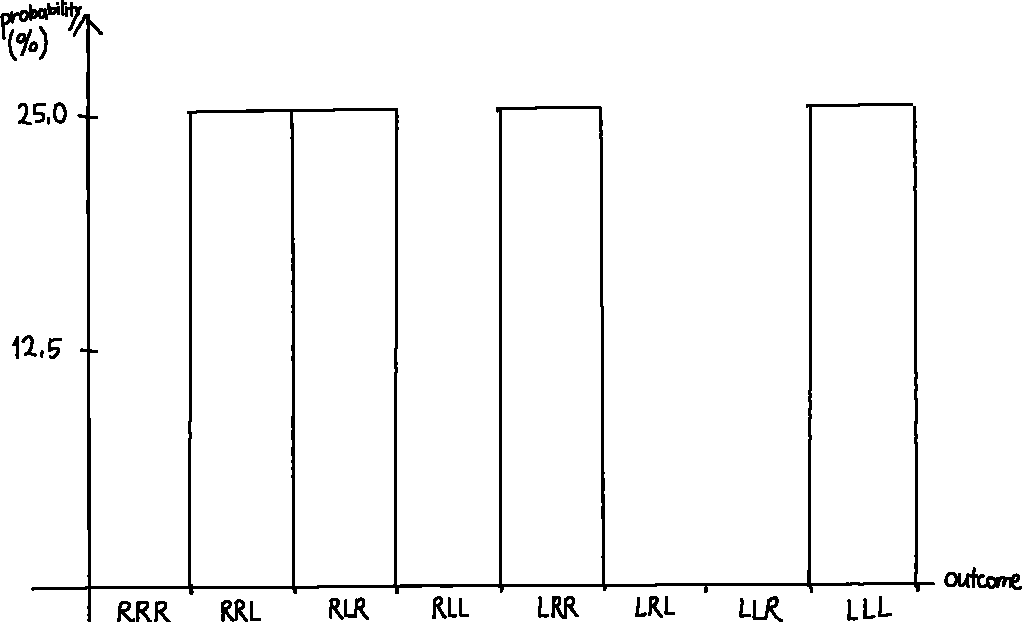
\includegraphics[width=.85\linewidth]{q6-histogram-local}
	\end{figure}
	\newpage
	Histogram for QM with phase flip error:
	\begin{figure}[H]
		\centering
		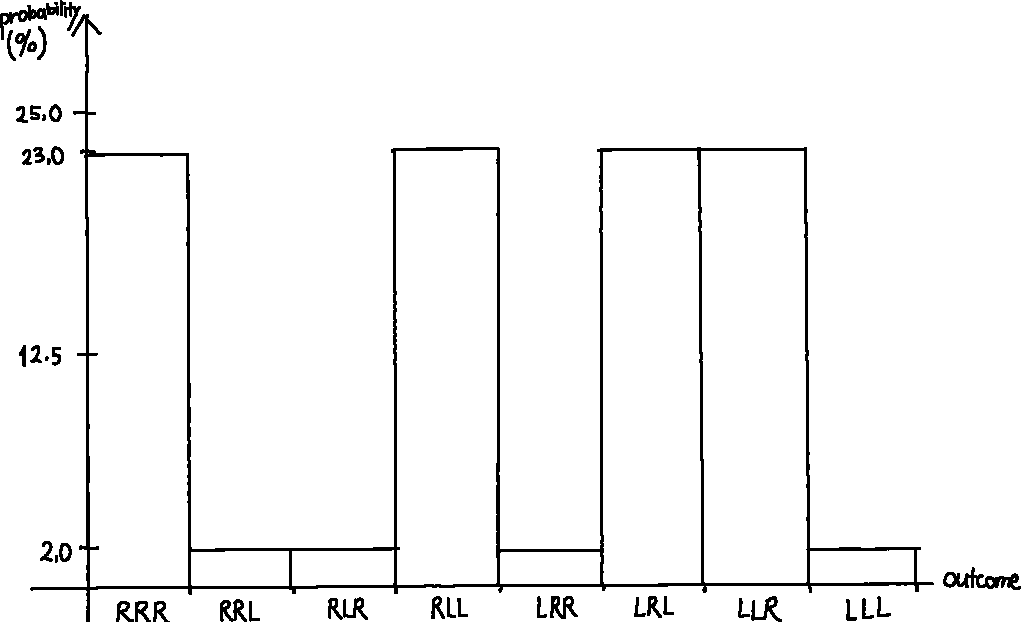
\includegraphics[width=.85\linewidth]{q6-histogram-qm}
	\end{figure}
\end{parts}